\documentclass[12pt, letterpaper]{article}

%%Paquetes
\usepackage{graphicx, subfig, float} %Insertar imagenes
\usepackage[export]{adjustbox}

\usepackage{authblk} %Autores de universidades
\usepackage{blindtext}
\usepackage{enumerate} %Numeraciones
\usepackage{booktabs, multirow, multicol} %tablas
\usepackage{amsmath, mathrsfs, amssymb} %math
\usepackage{siunitx} %unidades
\usepackage[parfill]{parskip} %no identación
\usepackage[spanish,es-tabla]{babel} %idioma

\usepackage[backend=biber,
    style=authoryear,
    natbib=true,
    sorting=nty,
    doi=false,
    isbn=false,
    url=false,
    giveninits=true,
    maxnames=2,
    maxbibnames=5
    ]{biblatex} %bibliografía
\addbibresource{libreria.bib}

%%Carpeta de figuras
\graphicspath{{figures/}}

%% Titulo
\title{Tutorial de Latex}

\author[a]{Autor 1 \thanks{\texttt{correo@gmail.com}}}
\author[b]{Autor 2 \thanks{\texttt{correo@gmail.com}}}
\author[c]{Autor 3 \thanks{\texttt{correo@gmail.com}}}

\affil[a]{Universidad 1}
\affil[b]{Universidad 2}

\date{\today}

%%

\begin{document}
\maketitle
\begin{abstract}
    \blindtext
\end{abstract}

\newpage
\tableofcontents
\newpage

\section{Introduction}\label{sec:intro}
\blindtext

\section{Section 1}\label{sec:subintro}
\blindtext

\subsection{Subsection 1}
\blindtext

\subsection{Listas}

Para definir listas usamos

\begin{itemize}
    \item Linea 1
    \item[!] Linea 2
    \item[*] Linea 3
\end{itemize}

Enumerar cosas

\begin{enumerate}[a)]
    \item Linea 1
    \item Linea 2
    \item Linea 3
\end{enumerate}

Combinar

\begin{enumerate}[a.]
    \item Linea 1
    \begin{itemize}
        \item Linea 1.1
        \item Linea 1.2
        \item Linea 1.3
    \end{itemize}
    \item Linea 2
\end{enumerate}

\section{Figures}\label{sec:figuras}
\blindtext. Figure \ref{fig:imagen 1}

\begin{figure}[h]
    \centering
    
\includegraphics[width=0.8 \textwidth]{image.jpg}
    \caption{Descripcion de la imgen}
    \label{fig:imagen 1}
\end{figure}

\blindtext. Figure \ref{fig:imagen 2}

\begin{figure}[H]
    \centering
    \subfloat[Descripcion grafica 1 \label{subfig:grafica11}]{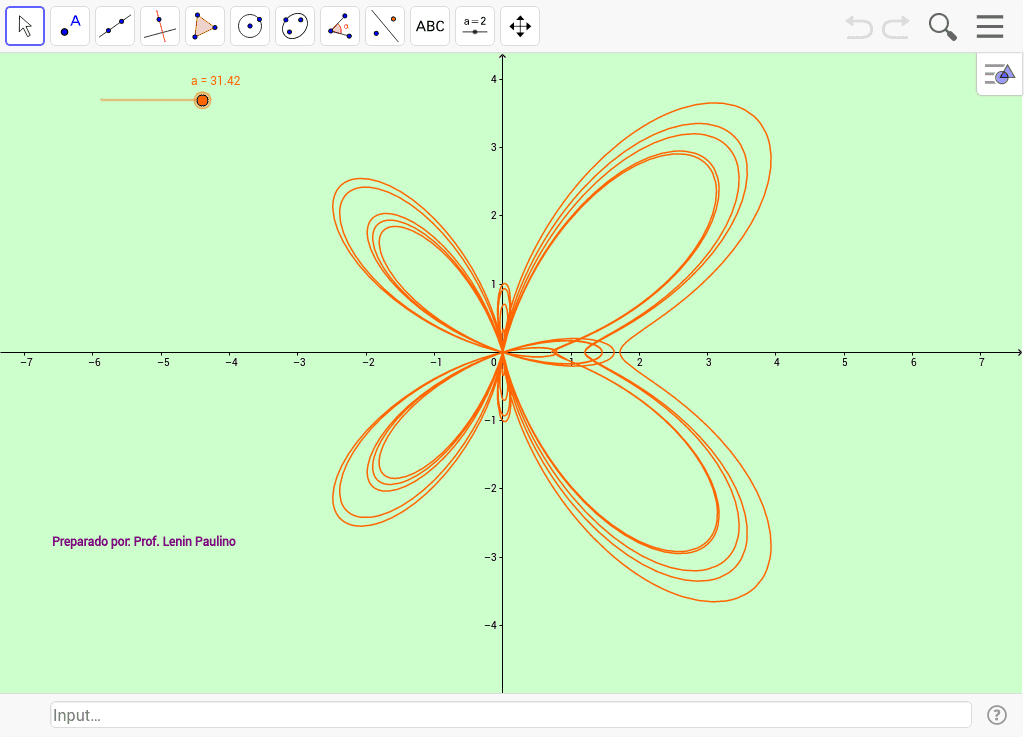
\includegraphics[width=0.4 \textwidth,valign=c]{grafica1.png}}
    \hfill
    \subfloat[Descripcion grafica 2 \label{subfig:grafica12}]{
\includegraphics[width=0.4 \textwidth,valign=c]{grafica2.png}}

    \caption{Descripcion de la imagen 2}
    \label{fig:imagen 2}
\end{figure}
\section{Tablas}

Como se menciono en la sección \ref{sec:figuras}

\begin{table}[h]
    \centering
    \begin{tabular}{cccc}
        \toprule
        A & B & C & D \\ \midrule
        1 & 2 & a & b \\ \midrule
        3 & 4 & c & d \\ 
        \bottomrule
    \end{tabular}
    \caption{Descripcion de la tabla 1}
    \label{tab:tabla1}
\end{table}

\blindtext

\begin{table}[H]
    \centering
    \begin{tabular}{lllll}
        \toprule
        \multirow{2}{*}{Models} & \multicolumn{3}{c}{Metric 1} & Metric 2\\
        \cmidrule{2-4} \cmidrule{5-5} \\
        {} & precision & recall & F-score  & R@10 \\
        \midrule
        model 1 & 0.67  & 0.8 & 0.729  & 0.75 \\
        model 2 & 0.8 & 0.9 & 0.847 & 0.85 \\
        \bottomrule
    \end{tabular}
\end{table}
\section{Ecuaciones}
Sabemos que $2+2=4$, lo cual es una suma. Pero en el caso de la multiplicación seria algo como:

$$ 2\cdot 2 = 4 $$

Para definir un entorno de ecuaciones utilizamos lo siguiente

\begin{equation}
    \int_{a}^{b} f(x)\cdot dx = 2x^2+\sin(x)
    \label{eqn:ecuacion1}
\end{equation}

\begin{equation*}
    \oint_{a}^{b} f(x)\cdot dx = 2x^2+\sin(x)
    \label{eqn:ecuacion2}
\end{equation*}

Si quiero citar la ecuacion anterior, lo hago con ref, y seria por ejemplo, la ecuacion \ref{eqn:ecuacion1}

\begin{align}
    %f(x) = 2x^3+\cos(x) + \ln(bx+3) +log(x^7) + \alpha\int_a^b g dx
    f(x) &= 2x^3+\cos(x) \\
         & \hspace{10pt} + \ln(bx+3) +log(x^7) \\ 
         & \hspace{10pt} + \alpha\int_a^b g dx 
\end{align}

Lo que utilizo para enumerar estas ecuaciones divididas

\begin{equation}
    \begin{split}
        f(x) & = 2x^3+\cos(x) \\
             & \hspace{10pt} + \ln(bx+3) +log(x^7) \\ 
            & \hspace{10pt} + \alpha\int_a^b g dx 
    \end{split}
    \label{eqn:ecuacion3}
\end{equation}

Para alinear ecuaciones en el centro

\begin{gather} %Recomendado en sistemas de ecuaciones
    f(x) = 2x^3+\cos(x) \\
         \hspace{10pt} + \ln(bx+3) +log(x^7) \\ 
         \hspace{10pt} + \alpha\int_a^b g dx 
\end{gather}

\begin{gather} %Recomendado en sistemas de ecuaciones
    2x+3=5 \\
    \sin(x) + x^4 = 3
\end{gather}

Para ingresar texto entremedio del entorno equation:

\begin{equation}
    \begin{bmatrix}
        a & b \\
        c & d
    \end{bmatrix}
    =
    \begin{bmatrix}
        1 \\
        2
    \end{bmatrix}
    \cdot
    \begin{bmatrix}
        3 & 4
    \end{bmatrix}
    \overset{\text{implicancia}}{\rightarrow}
    \lim_{x \to 2} f(x) in \mathbb{R}
\end{equation}

Algunas fuentes matemáticas son: $\mathbb{R}$, $\mathscr{R}$, $\mathfrak{R}$, $\mathcal{R}$, $\mathtt{R}$.

\newpage

Para definir una unidad a la mala podemos hacer;
\begin{equation}
    2 \ \text{mm}
\end{equation}

Para una mejor forma es utilizar el paquete siunitx

\begin{gather}
    2 \ \unit{kg.mol^{-1}} \\
    2 \ \unit{\kilogram\per\mole}
    \qty{2}{kg.mol^{-1}} %Recomendada
\end{gather}
\section{bibliografía y Citas}

\begin{itemize}
    \item Lo señalado por \cite{negusLinuxBible2015}
    \item Si queremos el año entre parentesis seria como \citet{negusLinuxBible2015}
    \item Todo entre parentesis: \citep{negusLinuxBible2015}
\end{itemize}

Para imprimir las referencias que hemos usado 

\printbibliography

Para imprimir las referencias que tenemos en el archivo.biber

\nocite{*}

\appendix
\section{Información complementaria 1}
\blindtext
\section{Información complementaria 2}
\blindtext


\end{document}
